% !TeX spellcheck = en_US
\documentclass[12pt,a4paper,twocolumn]{article}
\usepackage[utf8]{inputenc}
\usepackage[T1]{fontenc}
\usepackage{amsmath}
\usepackage{amssymb}
\usepackage{graphicx}
\usepackage{fancyhdr}
\usepackage[english]{babel}
\usepackage{geometry}
\usepackage[dvipsnames]{xcolor}
\usepackage[english]{babel}
\usepackage{hyperref}
\usepackage[style=numeric, url=true, doi=true, isbn=false]{biblatex}

\title{Clustering with a Convolutional Variational Autoencoders of Photoplethysmography Timeseries}
\author{Lorenzo Barsotti}

\addbibresource{bibliografia.bib}
%\bibliographystyle{plain}
\geometry{ margin=2cm}
\pagestyle{fancy}
\begin{document} \thispagestyle{empty}
	%\maketitle
	
	\twocolumn[{%
		\begin{@twocolumnfalse}
		\huge \bfseries Clustering with a Convolutional Variational Autoencoders of Photoplethysmography Time-Series
		\begin{flushright}
			\large \bfseries Author: Lorenzo Barsotti	
		\end{flushright}
		
			\begin{abstract}
				The purpose of this project is to analyze photoplethysmography data, with a Convolutional Variational Auto-encoder Neural Network. In particular we would like to see if there are some \emph{latent characteristics} that allow us to discriminate the biological age of a patient from its photoplethysmogram.
				
			\end{abstract}
		\end{@twocolumnfalse}
	}]

	\section{Introduction}
		The purpose of this project is to try to estimate the biological age of a patient, from its photoplethysmogram. A photoplethysmogram is the optically obtained signal related to the changes of volume in the blood vessels (section \ref{ppg_intro}). In order to perform the age estimation I used a database composed of about 4770 photoplethysmograms of as many patients, and a \emph{Convolutional Variational Auto-Encoder}. This is a particular case of \emph{Deep Neural Network} as it will be described in the section \ref{vae_intro}. To develop the Neural Network Tensorflow 2.9.0 \cite{tensorflow2015-whitepaper} was used.
	\subsection{Photoplethysmography}
		\label{ppg_intro}
		\emph{Photoplethysmography} is a technique that use light in order to detect changes in volumes in blood vascular vessels. A \emph{Light Emitting Diode} (LED), illuminates a high vascularized body part covered by a thin layer of skin, usually a fingertip, and a photodiode measures the amount of light transmitted or reflected. In the particular case of this project, the data were taken with camera module of smartphones: the LED illuminates a fingertip and the camera records the backscattered light. 
		A \emph{photoplethysmogram} (PPG)is the plot of the recorded data of the photodiode. It is a graph in which we are able to see how  of the blood vessels' volume change over time. Ideally the obtained time series is very regular and the present peaks corresponds to patient's  heartbeat (Figure \ref{fig:ppgexample}).
		\begin{figure}[h!]
			\centering
			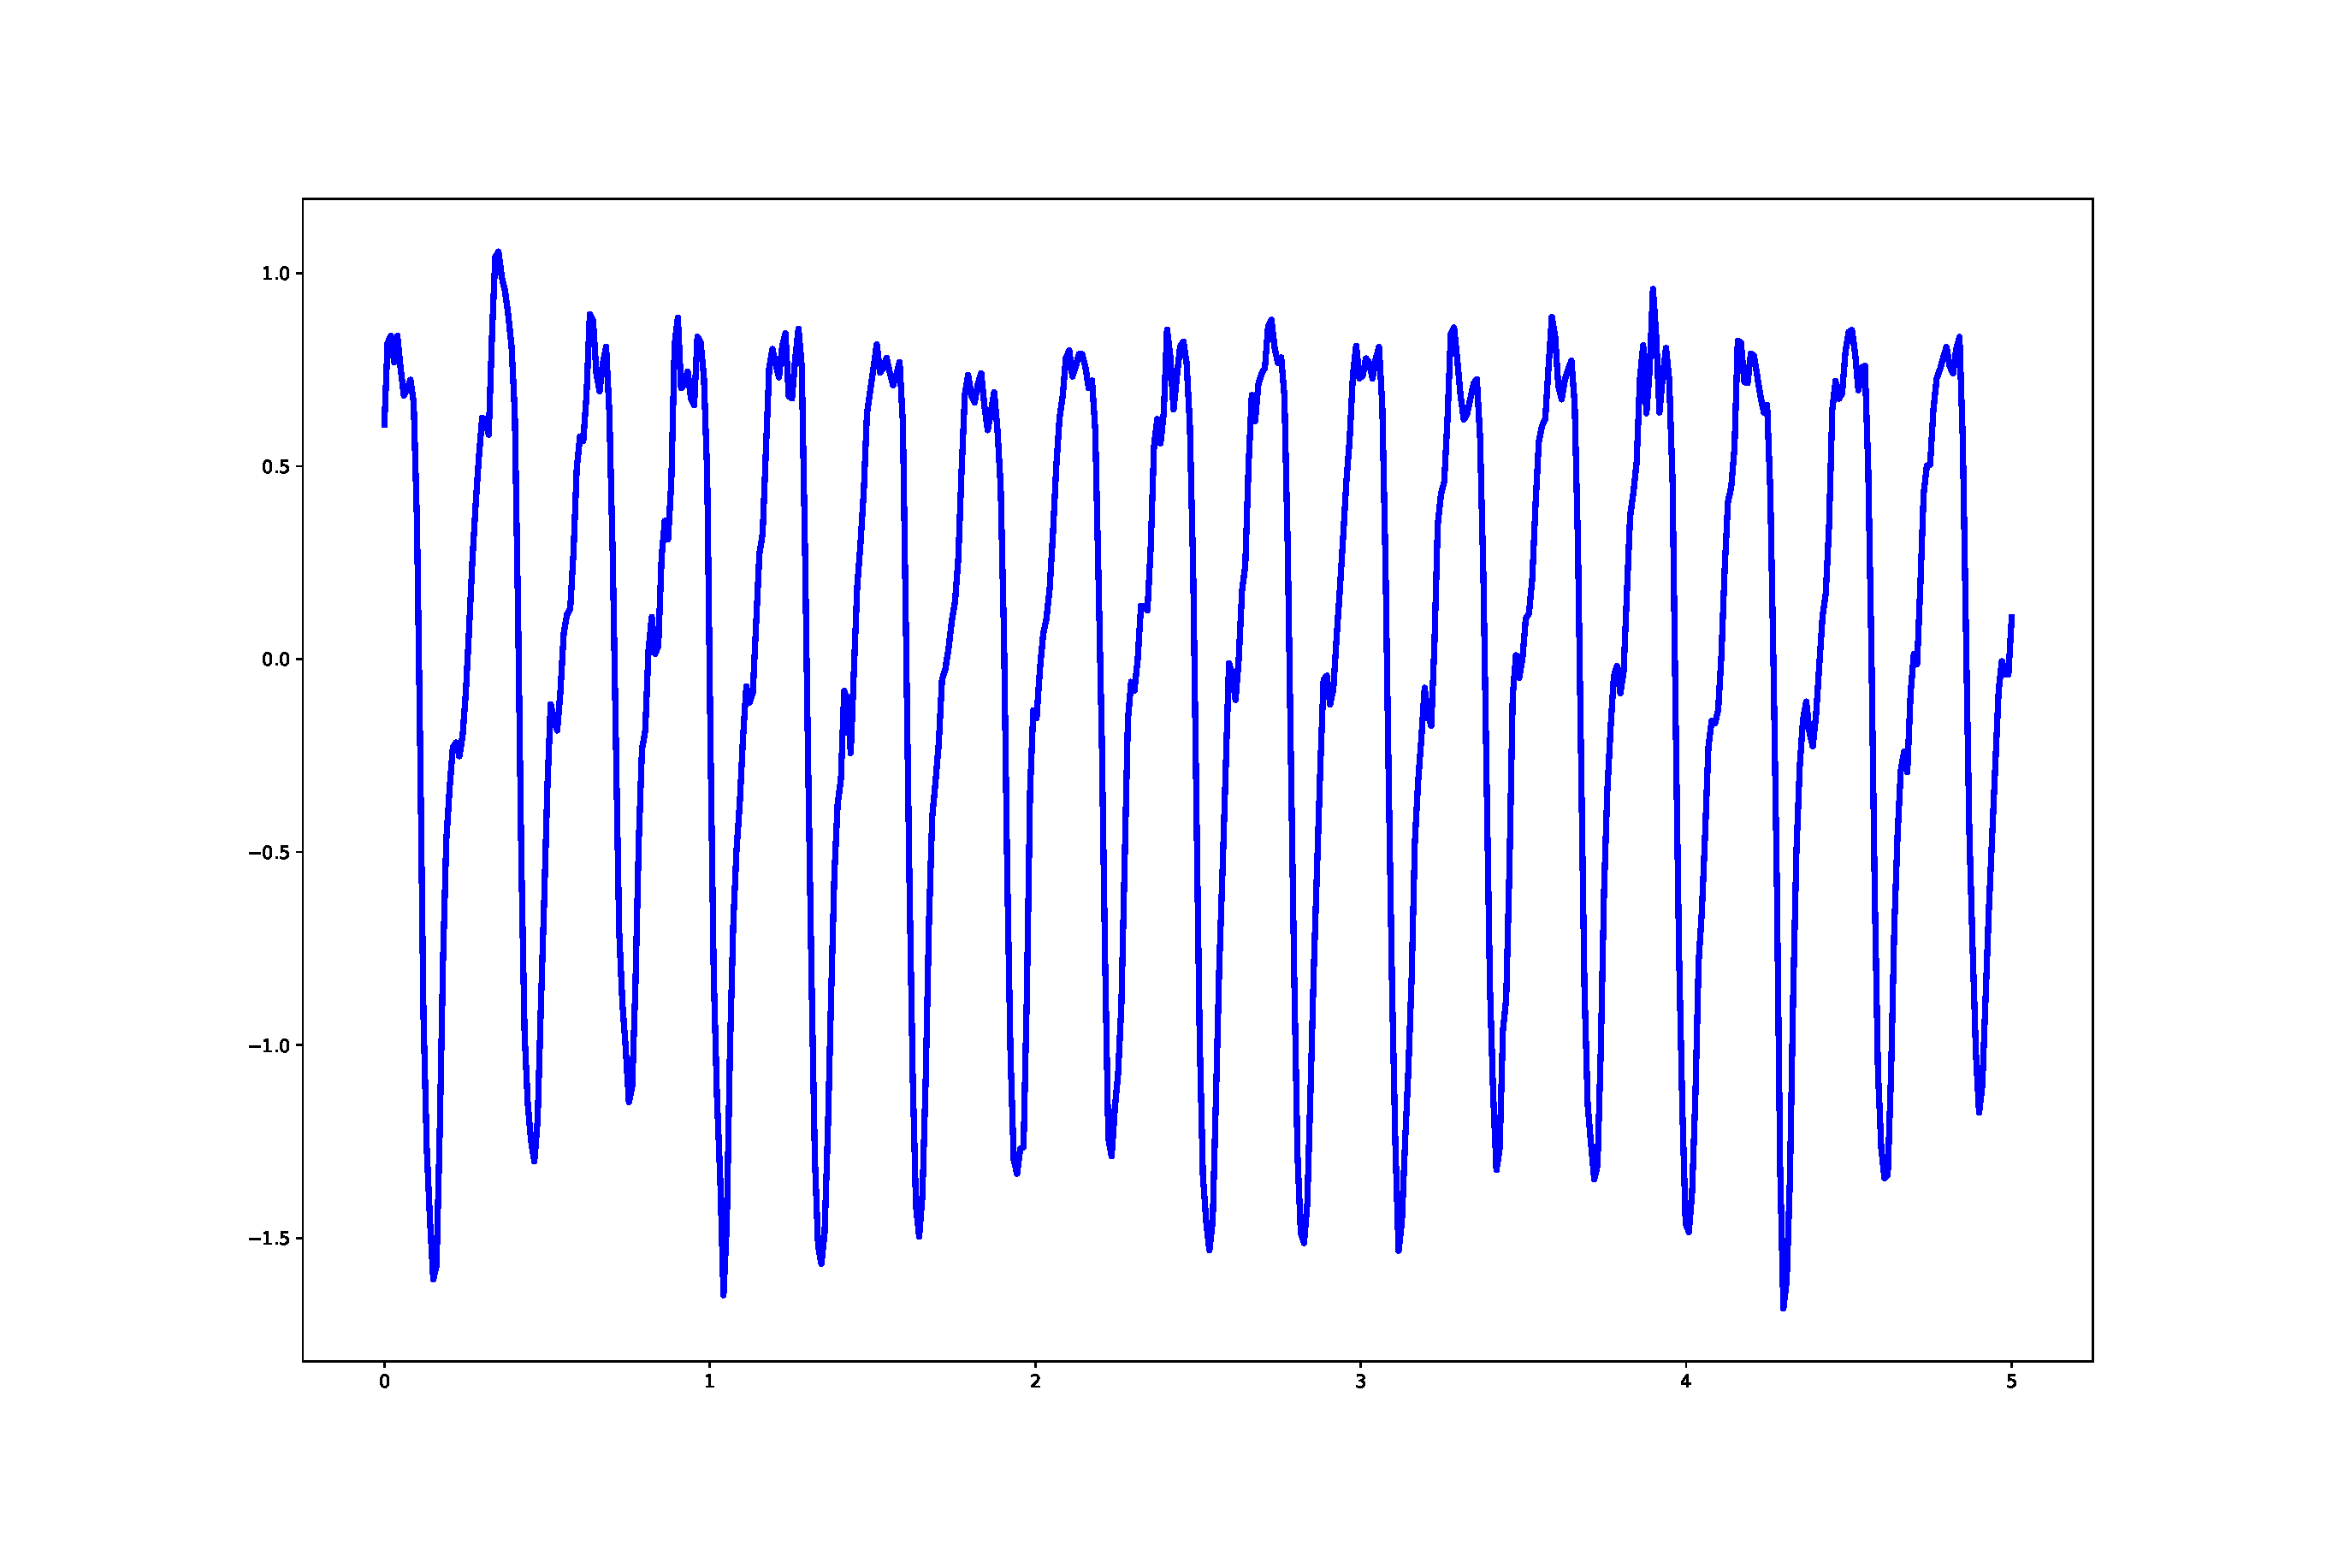
\includegraphics[width=1\linewidth]{images/ppg_example2}
			\caption{Example of a photoplethysmogram present in the database. The figure shows only the first part of the plot, that is much larger.}
			\label{fig:ppgexample}
		\end{figure}
		
		
		\section{The database}
			The database contains data coming from about 3600 patients. A PPG is saved in two arrays of the same length: the first one contains the signal, and the second one the time at which each signal of the first array has been recorded.  Two other important features used in this project and contained in the database, are the patient's age and a score related to the PPG quality.
			
			The other features of the database have not been used.
			\subsection{Preprocessing}
				The signals of the PPGs may not be always perfect: there could be some \emph{strange} peaks, or a very different behavior respect to the one in figure \ref{fig:ppgexample}.  This could be due to different factors, such as the pressure the patient push the finger with on the camera, or the position of the finger on the camera\dots These not \emph{well-behaving} PPGs must be removed from the database and, for this operation, the quality index is used. In this database lower the quality index is, the better the PPG is. For this reason I  set the a quality threshold at \colorbox{red}{0.005}, over the which the data are removed from the database. Doing this led to a number of usable PPGs to 3256. 
				A plate PPG has been removed manually because the quality threshold was not sufficeint to discriminate this particular PPG.
				
				\colorbox{red}{come sono presentati i dati}
				
		
			
		\section{Convolutional Variational Auto-Encoders}
			\label{vae_intro}
			\emph{Convolutional Variational Auto-Encorders} (CVAE) is an architecture of \emph{Deep Neural Network} (DNN). It can be used with different purposes, but in this project it has been used to perform an  \emph{unsupervised clustering}. This means that given the data, we would like to divide them in clusters depending on the age of the patients, without providing the corresponding labels during the training phase of the Neural Network. 
			
			\begin{figure}[h!] 
				\centering
				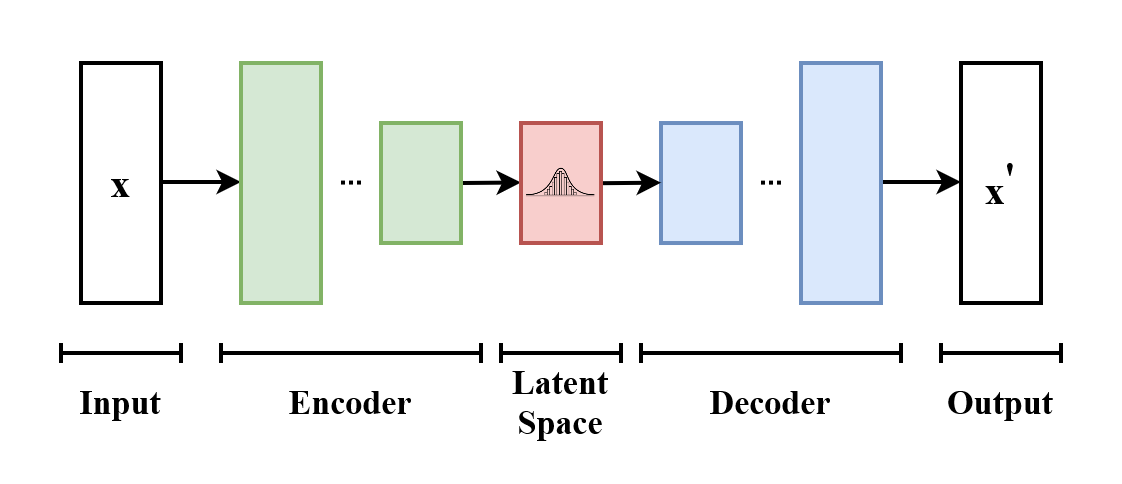
\includegraphics[width=1\linewidth]{images/VAE_Basic}
				\caption{Structure of a VAE. It is possible to distinguish the \emph{encoder} that, in the particular case of a CVAE, performs convolution operations, the \emph{ latent space}, in which the important information should be contained, and the \emph{decoder}, that try to reconstruct the output starting from the latent space and provide us the Neural Network output.}
				\label{fig:vaebasic}
			\end{figure}
			A \emph{Variational Auto-Encoders} (VAE) can be represented by the scheme in Figure \ref{fig:vaebasic}, where we can see that it is composed by several \emph{layers}. The data are provided to the input layer in the form of tensor, with a shape equal to (number of inputs, input height, input width, number of channel). This initial layer pass the data to the \emph{encoder}. The \emph{encoder} reduce the original information to simple distributions that should contain the same information of the original data (\emph{latent space}). Then a decoder is applied to the \emph{latent space} in order to reconstruct an output as much as similar to the input data.
			
			A CVAE  is a VAE in which, the encoder consist in perform convolution operations. A convolutional layer applies convolutions on the input and pass the result to the next layer. If the input of a convolutional layer are images,so if we consider a bi-dimensional input, the operation of convolution consist in bring together the information of a small number of pixel in an unique pixel. The pixel on which the convolution is performed, is determined by the \emph{kernel matrix}. Usually the \emph{kernel} is a square matrix with an odd-number of pixel per side. All the pixel in the original image are convoluted, with a \emph{kernel matrix} in a new single pixel. Once the boundary condition (\emph{padding}) and the \emph{stride} \footnote{The \emph{stride} parameter fixes how often we have to perform a convolution with the \emph{kernel matrix} respect to the length of the image. if the stride is 1, than the I repeat the convolution moving the source matrix of 1 pixel every time, if it is 2, I move the source matrix of two pixel, \dots} are fixed, the process must be repeated for every pixel of the original image. An example can be seen in the Figure \ref{fig:kernel}. 
			\begin{figure*}[t]
				\centering
				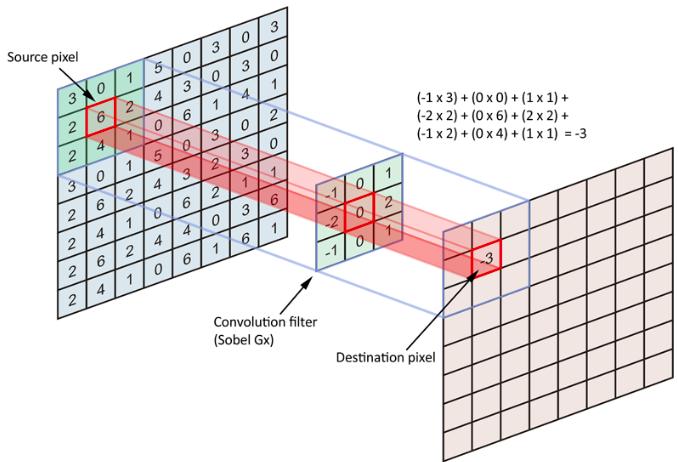
\includegraphics[width=0.7\linewidth]{images/kernel}
				\caption{Example of how a \emph{kernel} matrix convolution works. The source matrix is convoluted with the \emph{kernel} matrix. This lead to a number, that become the output value of a pixel}
				\label{fig:kernel}
			\end{figure*}
			
			The \emph{encoder}, maps the original image in a multivariate normal distribution, so its output is a vector, containing the mean and the standard deviation of the distribution. So with a bi-dimensional input, we would have a latent space composed by two vectors of this type, one for each dimension.  From the latent space, the VAE randomly samples the distribution, and extracts one point, that is fed to the \emph{decoder}, in order to reconstruct the output. This ensure that small differences in the latent space don't produce big differences as output. The mean and the variance are the learnable parameters. So if an input data point is to be mapped into a variable $z$, after the sapling from the distribution, it must follow: $$z = z_{mean} + \sigma\times\varepsilon$$ where the role of $\varepsilon$ will be seen in the subsection \ref{rep_trick}.
		
			\subsection{Loss Function}
			In the training of a VAE, we try to learn the parameter of a distribution. In order to do that, we use a loss function composed by two terms:
			\begin{itemize}
				\item \emph{Reconstruction loss}: that ensures the similarity between the input and the output.
				\item \emph{Regularization loss}: that helps to create a well-structured latent space and to reduce the overfitting of the training dataset.
			\end{itemize}
			For the \emph{reconstruction loss}, the \emph{Binary Crossentropy} was used
			In the VAE, the \emph{regularization term} is given by the \emph{Kullback-Liebler} (KL), \emph{Divergence}, that measures the distance between two distribution, the Gaussian one and the one of the latent space.
			\subsection{Reparametrization Trick}
			\label{rep_trick}
			The random sampling of the distribution introduce in the system stochasticity  
			\begin{figure*}[t]
				\centering
				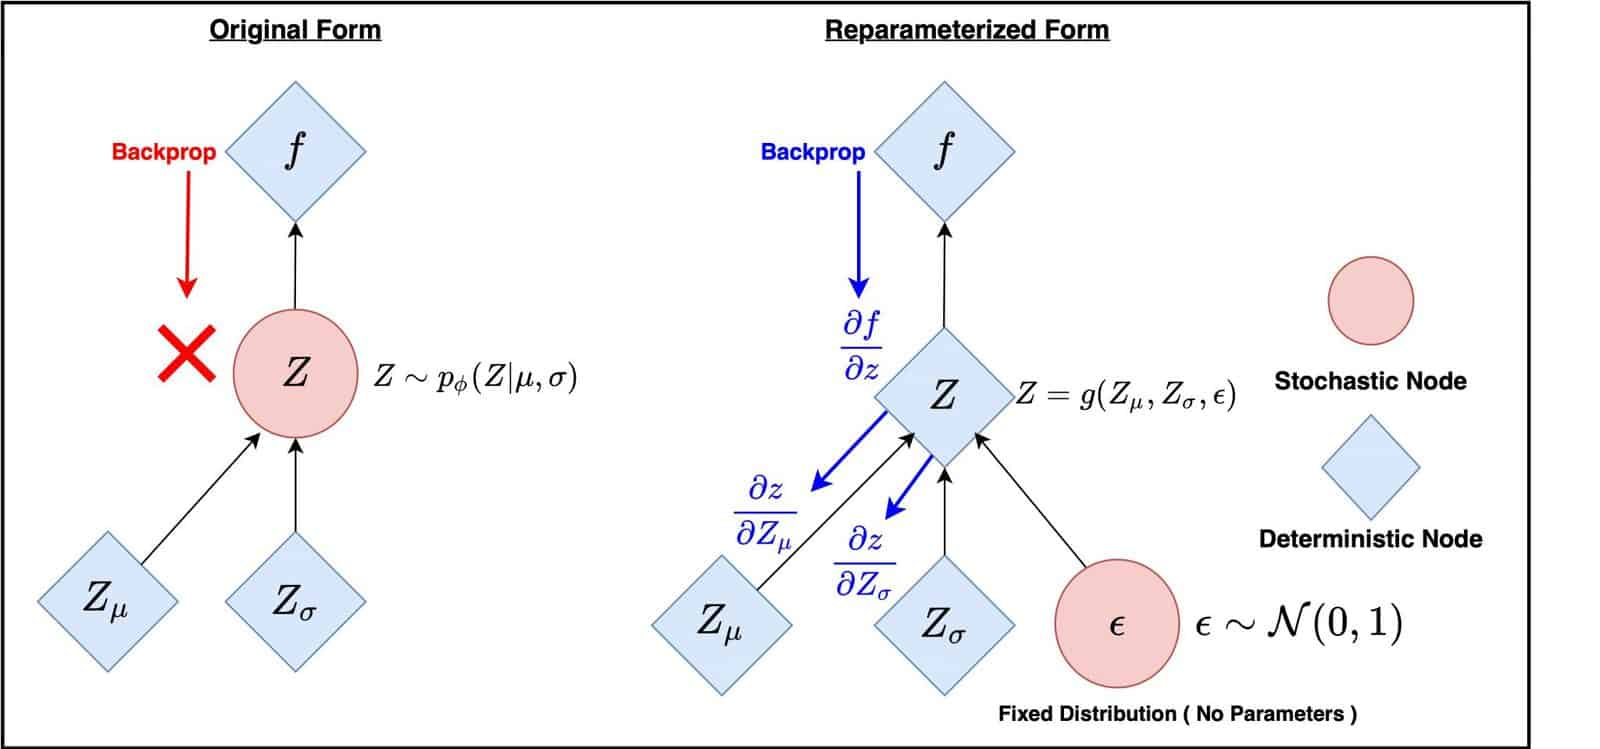
\includegraphics[width=0.7\linewidth]{images/reparam-vae-2048x959}
				\caption{}
				\label{fig:rep_trick}
			\end{figure*}
			
		\newpage
		
		\printbibliography
\end{document}